This chapter provides detailed specifications of the system.

%\section{Quantitative Design Specification \& Constraints}
%[]]]]]]
%The final product teaches self defense skills to users. It can teach up to 5 techniques which include a combination of blocking and punching. It captures motion using a single camera. The camera would be able to capture frames at a certain fps depending on the machine being used. 

%Anything lower than that means the resolution would suffer. In order to increase the frame rate the resolution would suffer. Currently the system is working on $92\times 92$ screen resolution, which means it has 92 by 92 pixels in each frame. The frames are images extracted from the video and each frame is processed. If the system is restricted to 10 fps. Therefore, we are currently unable to estimate high speed movements. The velocities need to be restricted with respect to the distance from the camera, such that it can be captured sufficiently in 10 frame each second. Another benefit of using OpenPose is that it gives us a confidence score. This confidence score tells us how accurate the pose is based on it machine learning model. The maximum accuracy is obtained when the object is nearly stationary and the camera focus is on the object, it is nearly 92\%. However, as the speed of the object increases and the object goes out of focus, this score decreases. 


\section{Design Concepts}

\subsection{Design Alternatives}

There are a number of alternatives to choose from in haptics and motion capture functionality. The following section explains the reason behind the choices made. 

\subsubsection{Haptic Feedback}

Haptic feedback comprises of impulse feedback and force feedback. Impulse feedback is used for sensation of interaction in the virtual world. It can be created using vibrotactile, EMS signal or a hybrid combination of both. Vibro-tactile reacts slowly and requires additional heavy hardware and a power supply. However, it does not require heavy calibration. EMS, on the other hand, minimises hardware and is much faster than turning on vibrational motors. With the right calibration EMS is much more realistic than vibrational motors, because it does not produce vibrating harmonics. The digital TENs machine, used in this project, does not produce any extra harmonics hence it gives a very fine tuned output. 

Force feedback is used for locking mechanism so that the user does not penetrate into the virtual character or objects. It can be given with an electromechanical structure with high torque motors or with EMS alone. Electromechanical devices are not comfortable to wear and a lot of hardware required, hence, EMS was used for force feedback.

\subsubsection{Motion Capture}

Motion capture can be done through a number of ways, namely, (a) leap motion, (b) kinnect and (c) camera/webcam. The first two work on infrared cameras. Leap motion was used by 2019 alumni and they highlighted the limitations of leap motion module. This device fails for our product since we needed a full body capture. kinnect is another alternative for full body motion capture, however, kinnect adds to the cost of the product. Furthermore, kinnect is not open source and extracting keypoints from it requires a lot of efforts and knowledge about its internal algorithms and source code of kinnect. However, camera is something most of the laptops and PCs already have, hence users will not need to buy it, and even if they have to, webcams are cheaply available. Camera is the cheapest hardware that can be used for motion capture. Although pose estimation through camera is much slower than kinnect, but algorithms can be deployed to make sure that without the loss of details, the net resolution is lowered such that frame rate is satisfactory enough. 

At a lower level we have to make a choice between different pose estimation libraries. We are currently using OpenPose, other options include Posenet and wrnchAI etc. wrnchAI performs far more better in speed as compared to openpose [cite], but it is not freely available. Posenet, is opensource but it has many different variants making it difficult to trace the actual documentation. We are using OpenPose because it is open source and has proper documentation available. An open source software has forums for help and is free to use. 


\subsection{Design Constraints}
\label{sub:designConstraints}
The haptic hardware, motion capture functionality and the computer machine used posed different types of constraints on the overall system. 

\subsubsection{Haptic Device Constraints}

There are a number of technological constraints that were identified in the initial phase of the project. One of the most major constraint in the system is the lesser degree of freedom in the EMS signal characteristics being used for haptics, which limits us to control the device active and inactive time periods, and the amplitude and the frequency of the signal to some extent. This could potentially be solved by creating a circuit of our own, however, it is not feasible because 

\begin{enumerate}
  \item prior to carrying out any tests on human subjects, it has to be certified through FDA to ensure human safety. 
  \item it is beyond the scope of this project.
\end{enumerate}

Therefore, the EMS device constraints are big challenges. There are a number hacks that can be used to get away with these technological constraints. To solve the device active and inactive time problem, we can use a sequence that schedules a move to happen only in the active window of the machine. Signal amplitude and frequency limitations can be solved using a haptic calibration scheme that will allow for more realistic impulse and force feedback. 


For medical safety, since we are restricting ourselves to use certified TENs machine only, we can only produce a certain types of signal parameters and wave characteristics. If we need a strong impact we cannot recreate it since these devices do not allow us to do so for safety. The maximum magnitude of current and voltage of wave are 0.08 mA and 90 V, the frequency is 157.1 Hz. This still provides a viable realization. Another safety concern with these devices is not to place electrodes near the neck, heart and face. Therefore we are restricting our project to just haptics on limbs, that too arms in specific. A way forward from this project could be to use legs and feet as well to teach moves that involve kicking and leg blocks too.


\subsubsection{Motion Capture Constraints}

Another major issue arises during realtime update of user's position in the software. The problem is that the speed of user's movement and the speed of pose estimation does not match. Openpose (in realtime mode) automatically skips some frames in between to process more recent frames. This frame skipping causes glitches in the user's virtual movement and also causes some serious problems such as user passing through a virtual wall, as the software couldn't identify a collision due to frame skipping. If, however, the realtime mode is turned off, then the user's virtual movements happen after a lot of delay than the user's original movements. 


Another issue regarding motion capture is the need for two cameras to capture depth for representing user in 3D virtual space. However, use of two cameras require a high knowledge of computer vision. It also adds to the cost because openpose requires both the cameras of a specific type and resolution for 3D pose estimation to work. The additional camera can also be an added burden to the hardware. This problem, however, can be solved using 3D pose baseline algorithms that can convert 2D pose to 3D pose, or by simply using the first frame from the user to estimate a relative depth of next frames from the user. 

\subsubsection{Computer Hardware Constraints}
Different types of computer hardware added to the speed and accuracy constraints. Pose estimation through openpose on a CPU machine with 3.8 GHz processing speed, 8 cores and 16 GB RAM provided far more accurate results than on a machine with GeForce 965M GPU of 2 GB RAM, 2.7 Ghz processing speed, 4 cores and 8 GB RAM. However, the speed of pose estimation increased by a factor of 10 - 12 approximately on a machine with GPU. Hence, there was a speed and accuracy trade-off depending on computer hardware. Speed is essential to realtime update of user's position in the virtual enviroment, and to provide feedback and score to the user of their performance no later than 1-2 minutes at max, while accuracy is essential to stable keypoint representation and better pose evaluation. There were also memory constraints posed by computer hardware. A GPU with 2 GB RAM limited the accuracy of the system to a very large extent, as it did not allow us go beyond $-1 \times 80$ net resolution due to insufficient memory to perform pose estimation on an image with more pixels. A lower net resolution of the input images to openpose resulted in pose estimation with lower precision and instability of keypoints. All the experiments related to this project are carried out on a machine with GPU, which means that the decreased accuracy of pose estimation heavily impacted the pose evaluation results. 

\section{Intellectual Contribution}

This project aims to introduce a virtual self defense trainer - a complete software solution with accessible hardware in a country like Pakistan where self-defense skills are a must to ensure safety. No other existing solution provides a complete guide with tutorials, practice and fight sessions for user to learn and practice together. 

Secondly, this project focuses on teaching self defense alone, which makes it concentrated and application specific unlike some of the existing solutions that have a broad range of applications. This product is designed to be able to give helpful user feedback, which is reflective of user's performance along with some tips to improve. This review is in natural language unlike some existing solutions which either do not give feedback at all or give feedback through haptic excitors and vibrations as described in section \ref{section:existingSolutions}. 

Our contribution also lies in our pose evaluation module which is entirely absent from the existing solutions and is very different from the existing literature on user pose evaluation. The mathematical models for scoring and classification were designed and finalized after a very rigourous experimentation and testing on our dataset. 

Another contribution is to exploit the self sufficiency of EMS for haptics \cite{EMSLopes}. Majority of the literature review consists of using hybrid of vibrotactile and EMS for tactile sensation or impulse feedback, and EMS and high torque motors coupled with electromechanical structure to give force feedback. However, this product offers a compact and easy to handle wearable with just comprises of electrodes and no motors. Although the testing and perception of haptic feedback is highly subjective, but sufficient experiments have been carried out to conclude that the perception is realistic enough. 

\section{Society, Economic, and Ethical considerations}

This project has its inspiration from societal problems and safety of citizens, especially women. It is being designed to make people feel good and positive about their bodies and feel confident when alone or in an unsafe company. Most of the countries including Pakistan have alarming rates of crime. Knowing basic self defense has been proven to protect people from unforeseen events. The project is aimed to be cheap enough as well for the common middle class families to afford it. One possible negative impact of this product is an increase in bullying and violence in schools, if underage kids are left unsupervised. It is important that the purpose of learning attacking skills is conveyed properly. 


The presented existing solutions are either expensive or not locally available, due to which people either don't know about the product or can not afford it. 
Our solution is cheaply available to any user who has a computer machine, and the hardware costs are low too, making it accessible for almost everyone. It can also result in empowering women at work, thereby increasing the workforce.  


EMS can be dangerous if used incorrectly, the ethics of this are reviewed and disclaimers have been appropriately provided in the manual in appendix A cite[][]. Data privacy is also considered and our project does not violate the privacy rights that a civilian has. The computation is local and if any data is needed in future for on server processing, then privacy measures will be deeply explored.

\section{Environment and Sustainability Considerations}

Our project takes considerations for environmental sustainability and aims to make a product that requires minimal hardware and maximum use of existing/recyclable resources. EMS devices and electrodes are the only requirement. The circuit needed is also very minimal. For motion capture the existing webcam in the laptop/PC is being utilized hence no overhead. It has a carbon footprint in only the connection with the computer's USB port, or utilizing the computer's charge, which is already in place. 


AEGIS consumes power from the user's laptop/desktop. Charging is not an issue and therefore no further batteries are used that could be harmful to the environment as well.
The hardware can work for many years if handled properly, requiring only the maintenance of electrodes. This could be done via ultrasound gel which is easily and cheaply available. The cloth used is elastic fabric, which is used medically. Our solution also has a lower carbon footprint compared to existing solutions. It is environmentally very friendly.

\section{Specific requirements}

\subsection{Functional Requirements}

This section describes each function/feature provided by our system. These functions are logically grouped into modules based on their purpose/users/mode of operations etc (as per our system). A functional hierarchy may look like:

\begin{outline}

  \1 Login/Signup Module
  \2 The user should be able to login to the system
    \3 The software should automatically and immediately validate user credentials against the database system
    \3 After verification, the software should grant access to the user’s account only if all the credentials of the user match. 
  \2 The user should be able to create a new account (Signup)
    \3 The software should write the credentials for this new account in the database.
    \3 After storing the credentials, the software prompt the user to verfify their email address, and proceed to the login screen.
  \2 The user should be able to change their password.
    \3 The software should update the password entry for the corresponding username in the database. 

 \1 Interface requirements
  \2 If the user has access to the account, they should be able to see the home screen of the software. The home screen will mainly give user the option to select between two options \textit{Training} and \textit{Fighting}.
  \2 The training session contains numbered lessons. Each lesson contains tutorials and practice sessions. 
  \2 The fighting session also contains numbered fights. Each fight $x$ requires the user to know the techniques included in lesson 1 till lesson $x$. A fight session is like a game in which user fights with the avatar. The avatar and the user, both have their health bars, which decreases if any of them fails to defend themselves against the opponent's attack. The fight session ends if either the user or avatar’s health bar gets empty. 
  \2 The user should be able to view the unlocked lessons. Lesson 1 will be unlocked by default and completing a lesson will unlock the next one. 
  \2 The user should be able to start the fight sessions of the corresponding unlocked lessons. 
  \2 The user should be able to view all the tutorials of an unlocked lesson. These tutorials are videos that teach the user a specific technique of self-defense. 
  \2 The user should be able to practice any of the tutorials from the unlocked lessons. This practice session is only of a specific technique which the tutorial teaches. 
  \2 If the user selects the haptic option for practice and fight session, they should be able to feel the interaction with the avatar after properly calibrating all the signal parameters.
  \2 The user should be able to see the feedback generated after a practice session ends.
  \2 The user should be able to start a fight session of an unlocked lesson.
  \2 The user should be able to see the feedback generated after a fight session ends.
  \2 The user should be able to see suggested tutorials to practice after fight session. These tutorials are the areas in which user needs improvement. 
  
 \1 Practice Session
   \2 If the user chooses to practice a specific tutorial, the avatar will attack, requiring the user to perform that specific technique which the tutorial teaches.  After the avatar is done performing the attack, the practice session will end giving detailed feedback to the user of his performance. 
 
 \1 Pose Detection Module
   \2 If the user selects to practice a tutorial or fight with avatar, the system should be able to extract stick figure data of their movement via OpenPose and a webcam/camera.
 \1 Feature Extraction Module
 `\2 The system should extract the required features like velocity, acceleration, torso distance, kinetic energy etc. to be used for further analysis.
 \1 Pose Classification Module
  \2 Since the user is just practicing a single known move in practice session, the system does not need to classify the performed pose for practice session. For fight session, however, in order for pose evaluation to take place, we first need to classify the pose into one of the stored poses.
  \2 In fight session, since the user will be performing several moves at the same time in response to avatar’s attacks, each performed move by the user will be classified. After classification of each performed move, each will go through pose evaluation module to get feedback on their moves separately rather than one combined feedback. 
  
 \1 Pose Evaluation Module
  \2 The system should be able to evaluate the different moves performed by the user in practice and fight sessions.
    \3 The system should use the extracted features to calculate a score indicating how well the user performed a particular move by comparing it against the benchmark.

 \1 User Feedback Module
  %\2 The user should be able to get visual feedback
  %  \3 The visual feedback consists of difference between the performed pose (stick figure) at an instant (the time instant where user made a mistake) and the stored pose (stick figure). The stored (correct) pose will be displayed in green and the part of the user’s pose will be displayed in red which do not properly align with the stored ones.  
  \2 The user should be able to get textual feedback 
   \3 The textual feedback will consist of a natural language feedback, which will tell the user what he/she lacked and how they can improve. 

 \1 Adaptive Teaching Module
  \2 The tutorials suggested by the system for more practice should be based on the low pose evaluation scores. 

 \1 Haptic Feedback Module
  \2 The system should be integrated with the haptic hardware.
  \2 The user should be able to calibrate the signal parameters for haptics that best comforts them.
  \2 The user should not penetrate into the avatar’s body.
  \2 The user should feel the impulse feedback on his arms and fists. 
\end{outline}

% --- The above is to be modified as per your project, e.g. a flat list if your system has limited functional requirements.

\subsection{Non-functional Requirements}
Following are the non-functional requirements of our system.
\subsubsection{Compatibility}
Software should be able to work on any laptop or computer with a camera.
\subsubsection{Usability}
The software should be user friendly and easy to navigate; no prior knowledge in the domain of Computer Science or self defense should be required for the user to experience the environment. 
\subsubsection{Modifiability}
The software can be expanded to other skills and functionalities, for instance additional defense techniques, if needed.
\subsubsection{Credibility}
Users can change their login password anytime they want; the new credentials must be updated in the database. 
\subsubsection{Integrability}
All components, whether they be software or hardware, should be integrated efficiently to ensure the smooth flow of the program when it is run. 
\subsubsection{Independability}
Besides being able to work as a complete, integrated project, the different components within the hardware should be able to function independently as well. For example, if one component of hardware fails, the other components should keep working. 
\subsubsection{Performance}
The program should provide a quick response time. It will be receiving user performance data in real-time and should respond to the user with relevant feedback in 1-2 minutes at max. 
\section{External Interfaces}

\subsection{User Interface Mockups}
This section includes our mockup screens and briefly explains them. Figure \ref{fig:startingScreens} shows our screens for login/signup functionality. The software launches with a logo screen shown in figure \ref{fig:logo} which slowly fades out to display the login screen in figure \ref{fig:login}. If the user doesn't remember their password, they can change it through the change password screen in figure \ref{fig:password}. If the user does not have an account already, they can make a new account through the signup screen shown in figure \ref{fig:singup}.


    \begin{figure}
  \subfigure[Logo Screen]{% 
    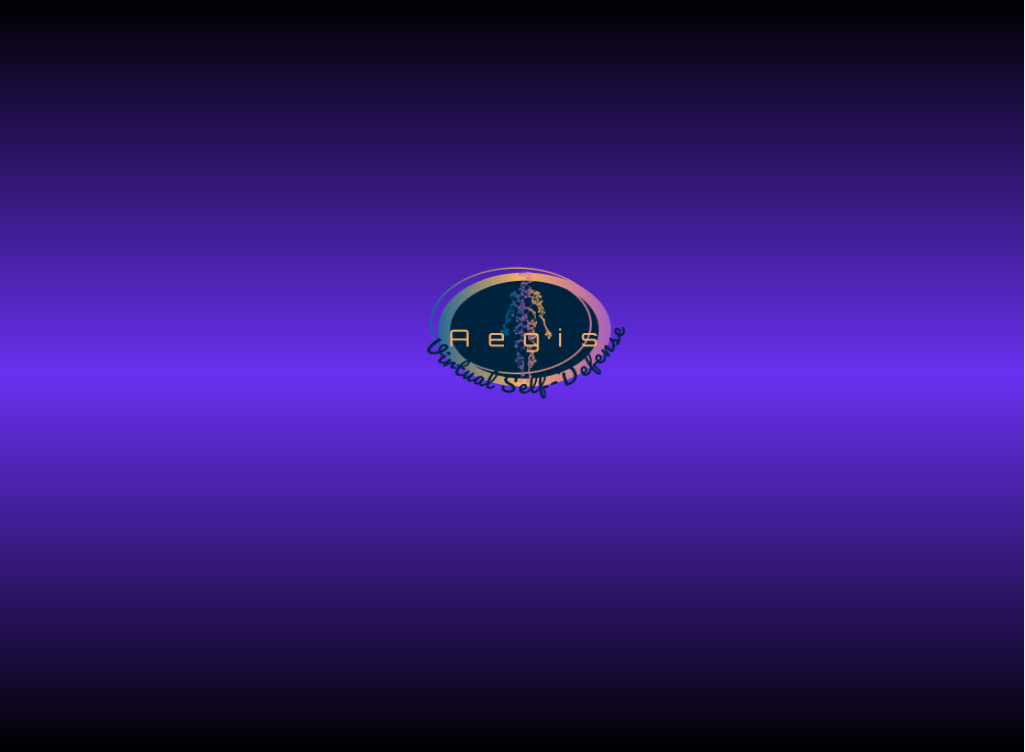
\includegraphics[scale=0.25]{images/Mockups/logo.png} \label{fig:logo} 
  } 
 \quad 
  \subfigure[Signup Screen]{% 
    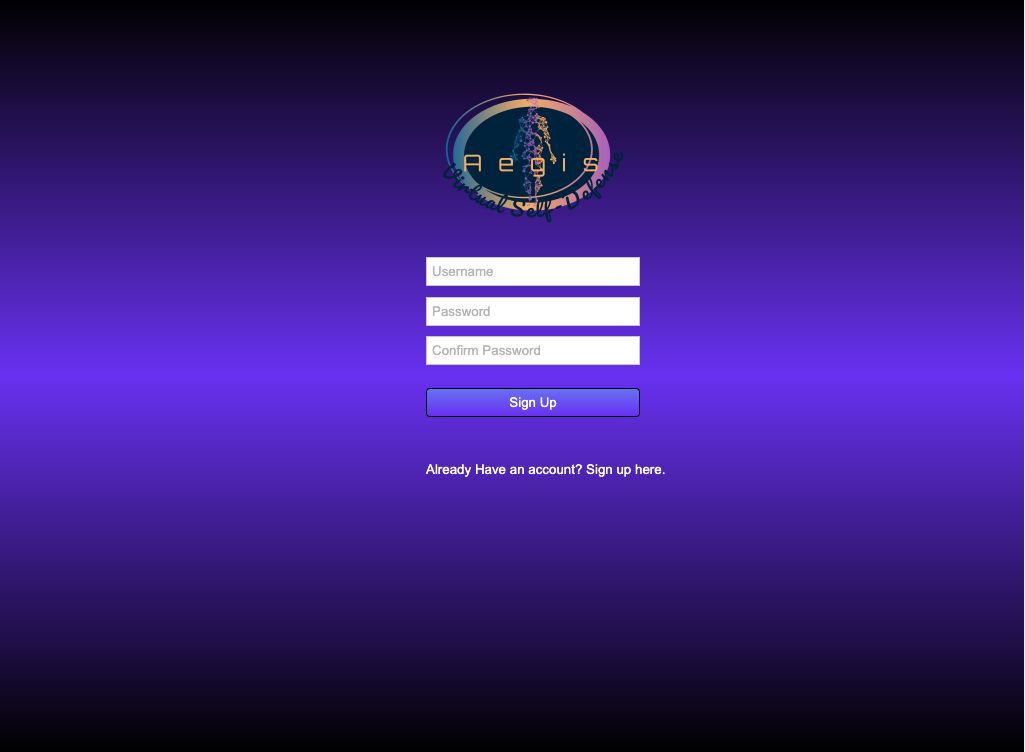
\includegraphics[scale=0.25]{images/Mockups/signup.png} \label{fig:singup} 
  } 
  \quad 
  \subfigure[Login Screen]{% 
    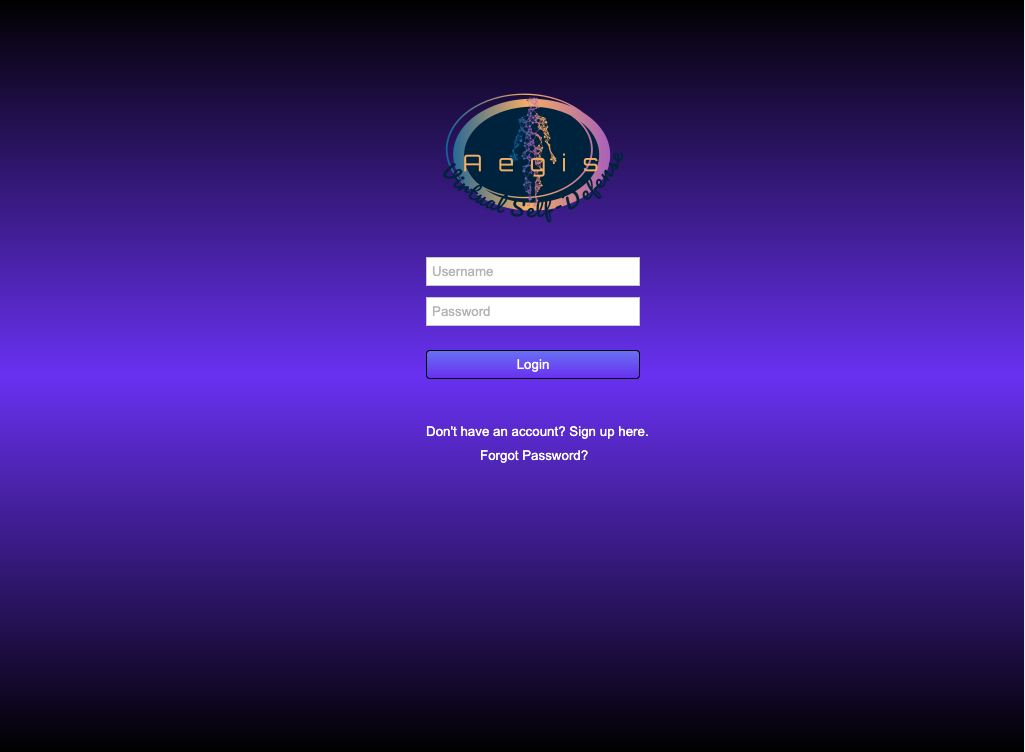
\includegraphics[scale=0.25]{images/Mockups/login.png} \label{fig:login} 
  }
  \quad 
  \subfigure[Change Password Screen]{% 
    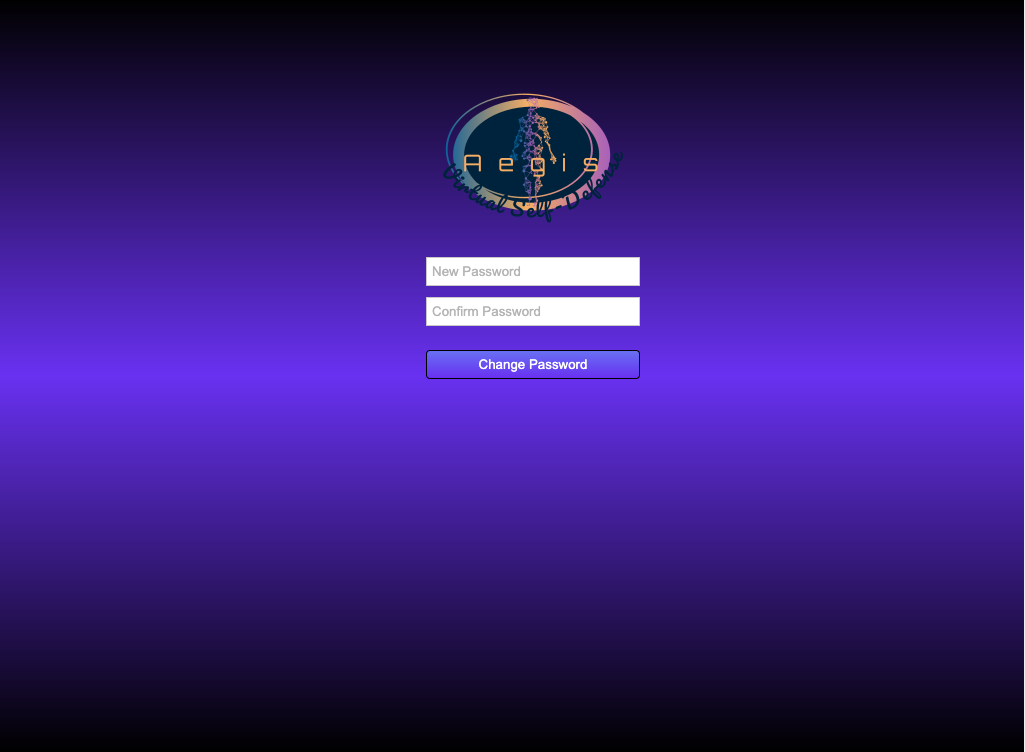
\includegraphics[scale=0.25]{images/Mockups/password.png} \label{fig:password} 
  }
  \caption{Login/Signup Functionality} 
  \centering
  \label{fig:startingScreens}
\end{figure}


Figure \ref{fig:homeTut} shows multiple screens related to home and \textit{Lesson 1} videos. After the user has been granted access to their account, home screen as shown in figure \ref{fig:home} is displayed. This screen gives user the option to choose between \textit{Training} or \textit{Fight} mode. Figure \ref{fig:lesson} shows the screen from where the user can navigate to introductory session of \textit{Lesson 1}, its tutorials and fight session. Screen in figure \ref{fig:intro} will guide the user what they will be learning in \textit{Lesson 1} which will be an animated video. Screen in figure \ref{fig:tutorial} will also display an animated video to the user guiding how a certain technique (specific to that tutorial) should be performed. 

    \begin{figure}
  \subfigure[Home Screen]{% 
    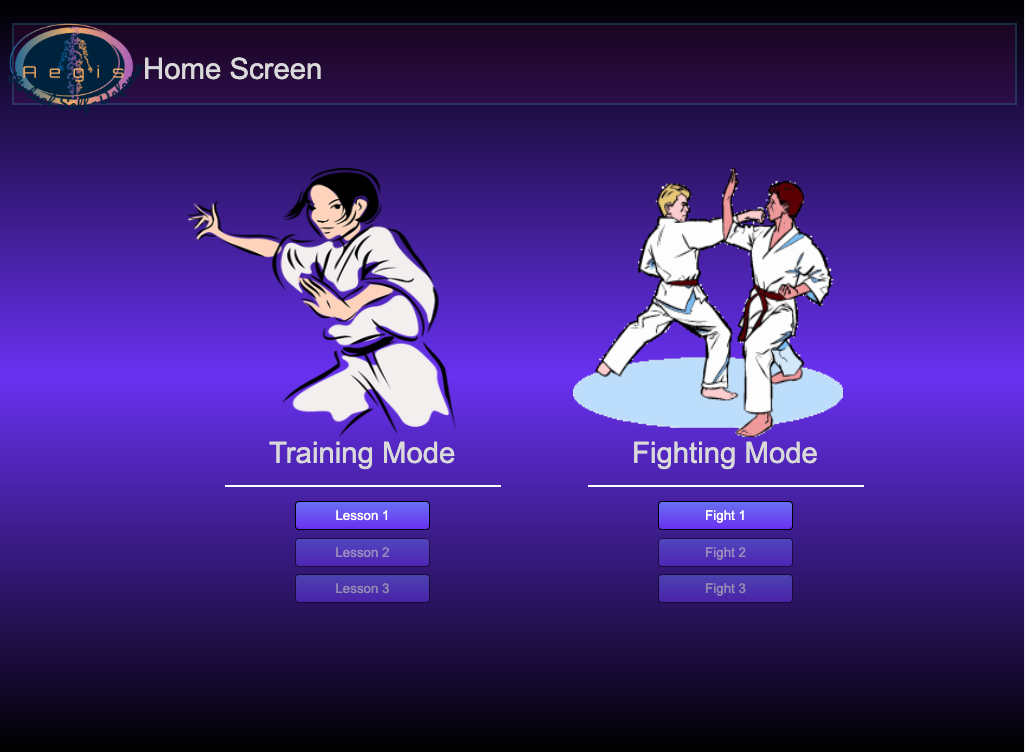
\includegraphics[scale=0.25]{images/Mockups/home.png} \label{fig:home} 
  } 
 \quad 
  \subfigure[Lesson I Screen]{% 
    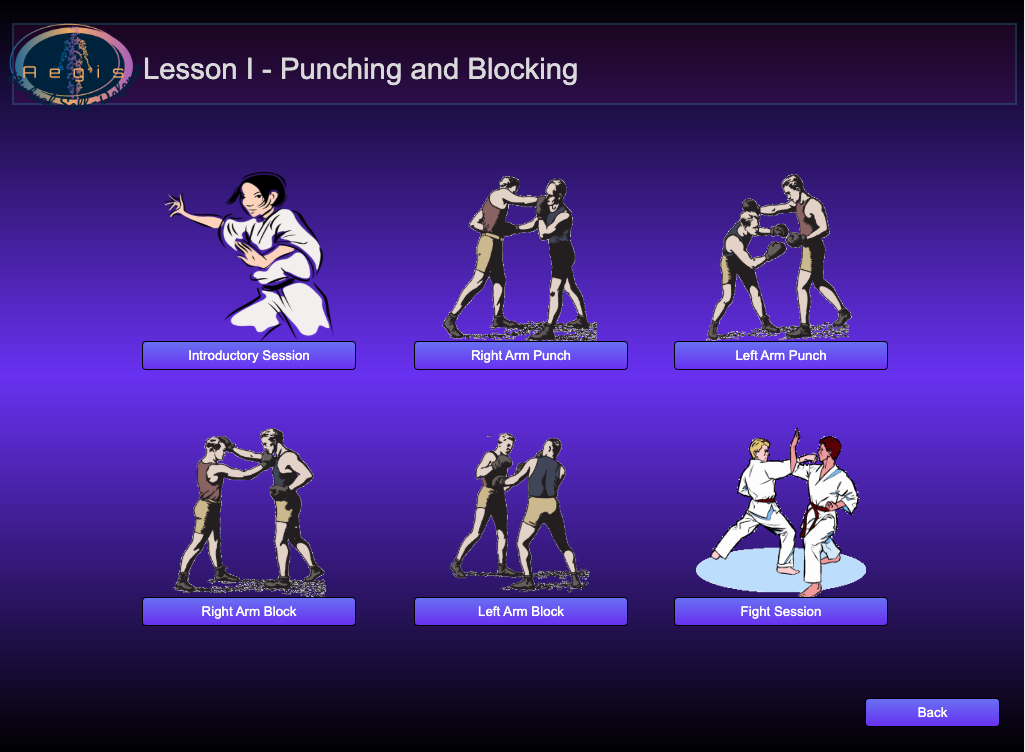
\includegraphics[scale=0.25]{images/Mockups/lesson.png} \label{fig:lesson} 
  } 
  \quad 
  \subfigure[Lesson I: Intro Screen]{% 
    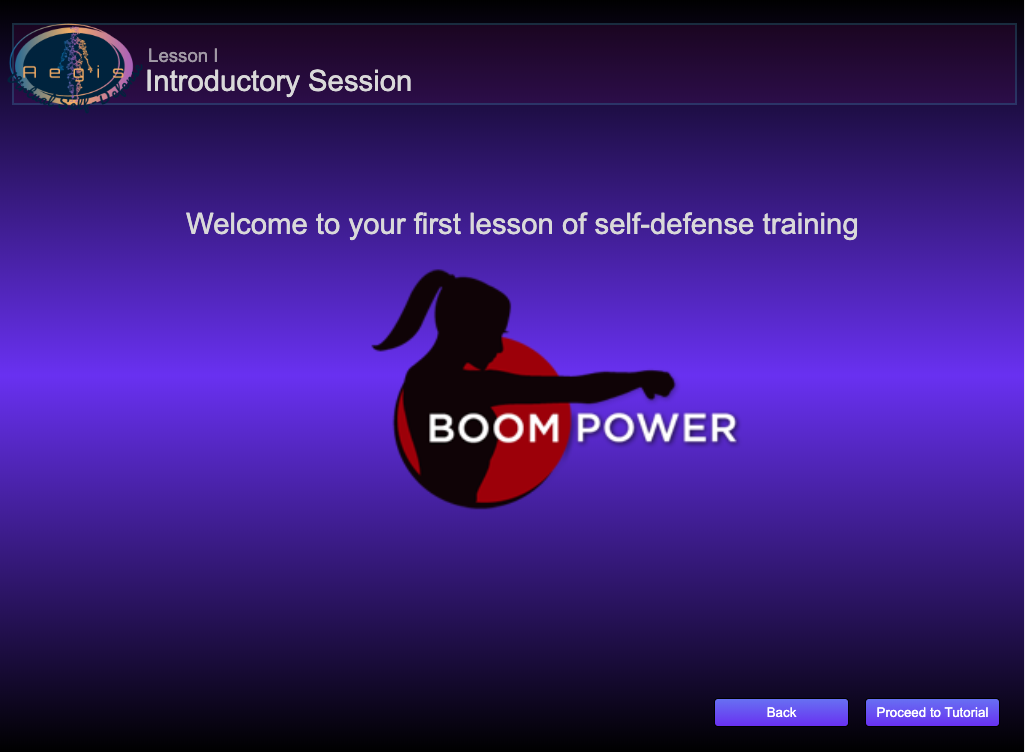
\includegraphics[scale=0.25]{images/Mockups/intro.png} \label{fig:intro} 
  }
  \quad 
  \subfigure[Lesson I: Tutorial I Screen]{% 
    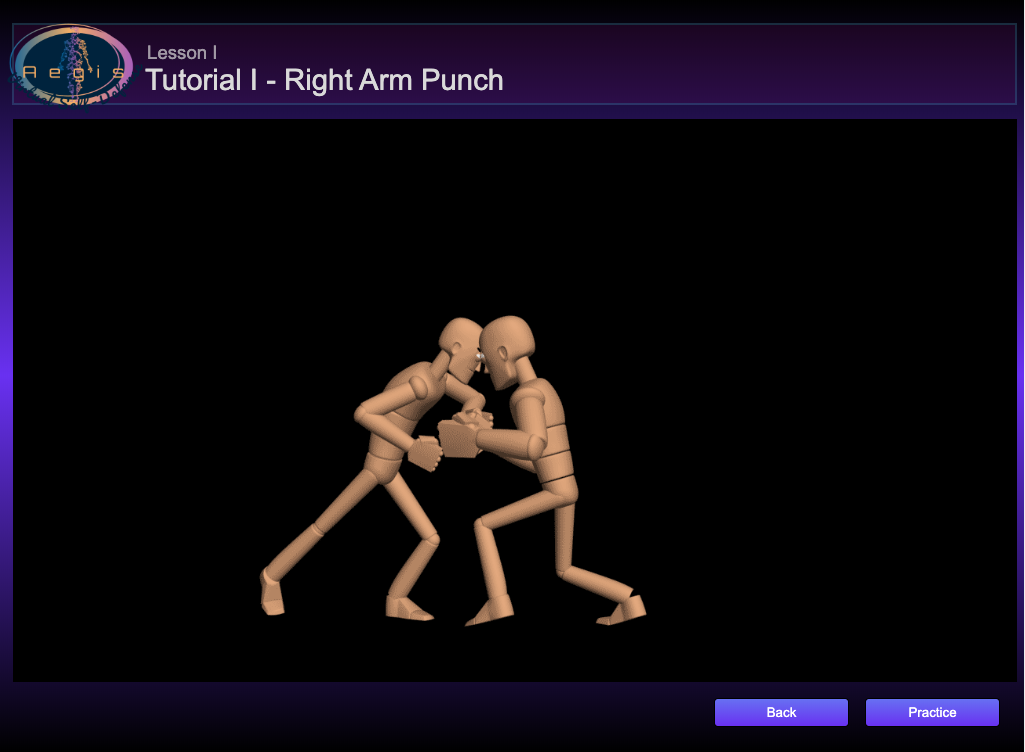
\includegraphics[scale=0.25]{images/Mockups/tutorial.png} \label{fig:tutorial} 
  }
  \caption{Home Screen and Tutorials} 
  \centering
  \label{fig:homeTut}
\end{figure}


Figure \ref{fig:practiceFight} shows screens related to \textit{Practice} and \textit{Fight} sessions. If the user chooses to practice or fight, they will first be asked if they want to do so with a haptic suit as shown in figure \ref{fig:dialogBox}. If the user responds in positive, they will be guided to put their haptic suit on (as shown in figure \ref{fig:haptic}) and will be prompted to calibrate the frequency and amplitude of the haptic signal that they prefer. Figure \ref{fig:practice} and \ref{fig:fight} shows the practice and fight sessions screens. These sessions will start when user clicks the \textit{Start} button. After the session has ended, a feedback report is available on the left.


\begin{figure}
  \subfigure[Haptic Screen]{% 
    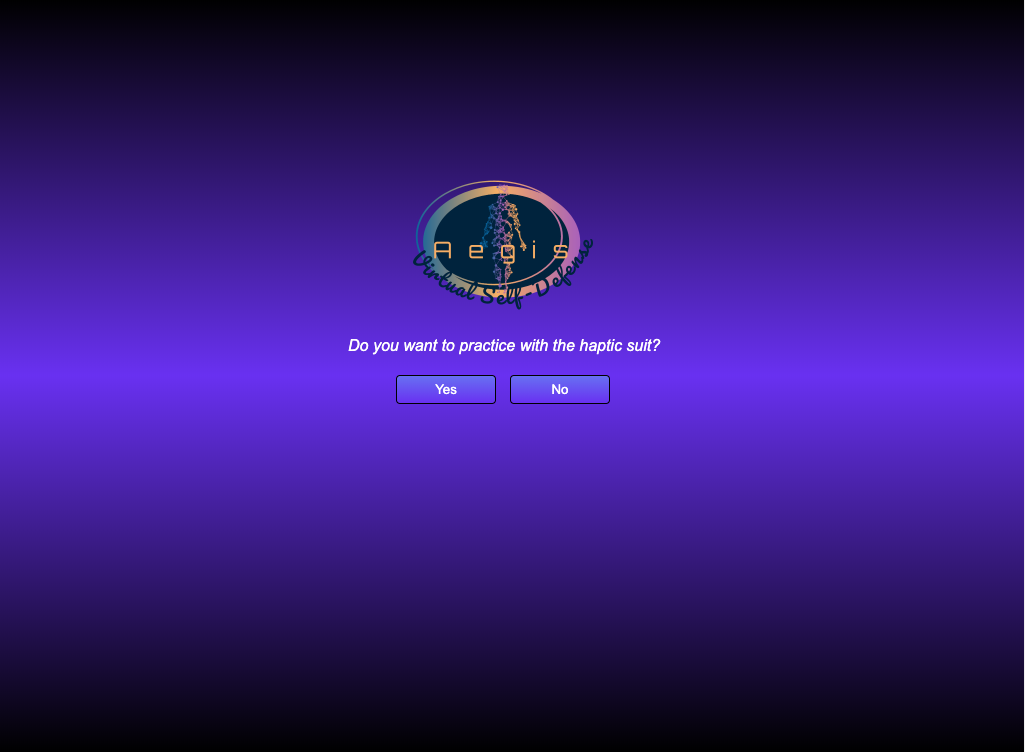
\includegraphics[scale=0.25]{images/Mockups/hapticDialogBox.png} \label{fig:dialogBox} 
  } 
  \quad 
  \subfigure[Haptic Calibration Screen]{% 
    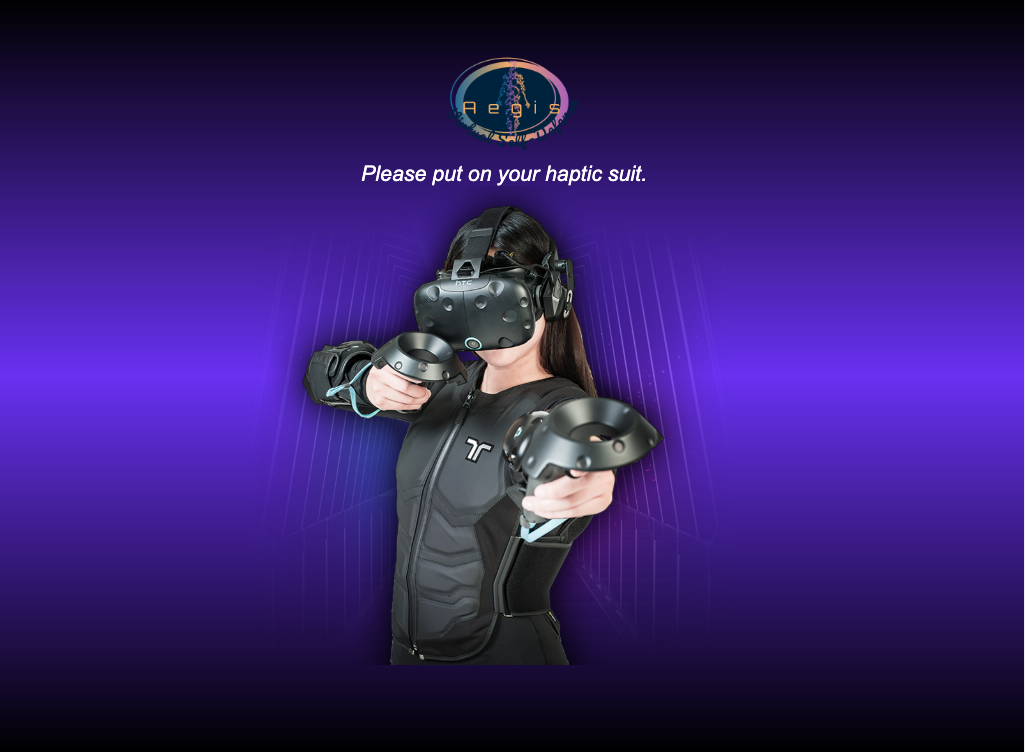
\includegraphics[scale=0.25]{images/Mockups/haptic.png} \label{fig:haptic} 
  } 
  \quad 
  \subfigure[Lesson I Tutorial I: Practice Session Screen]{% 
    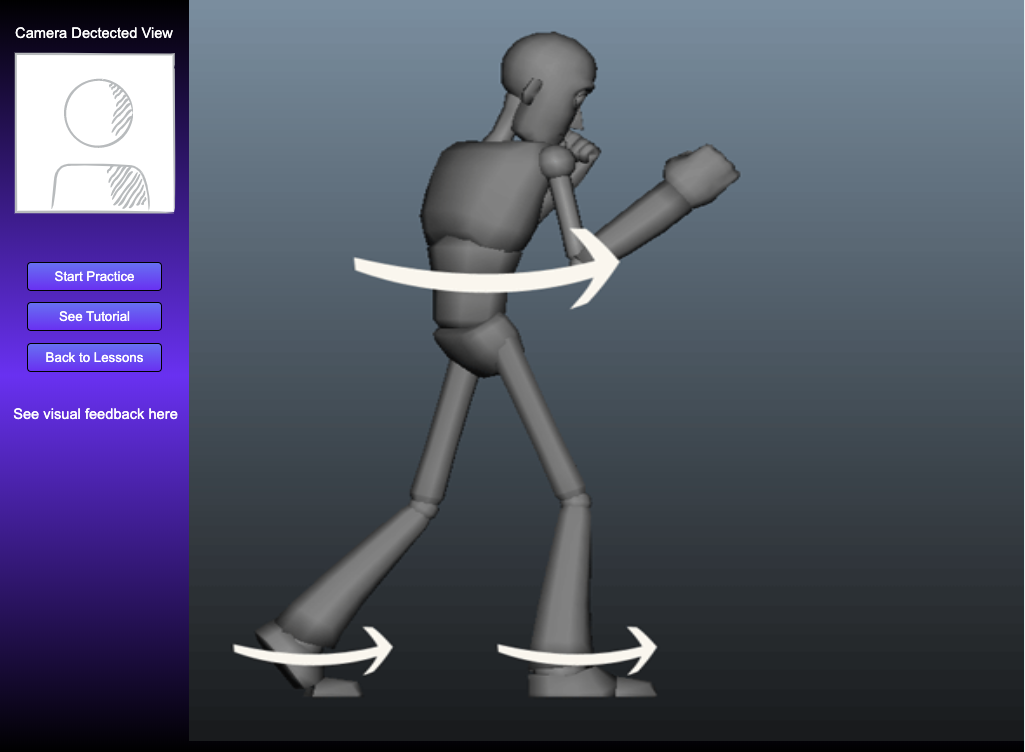
\includegraphics[scale=0.25]{images/Mockups/practice.png} \label{fig:practice} 
  }
  \quad 
  \subfigure[Lesson I: Fight Session Screen]{% 
    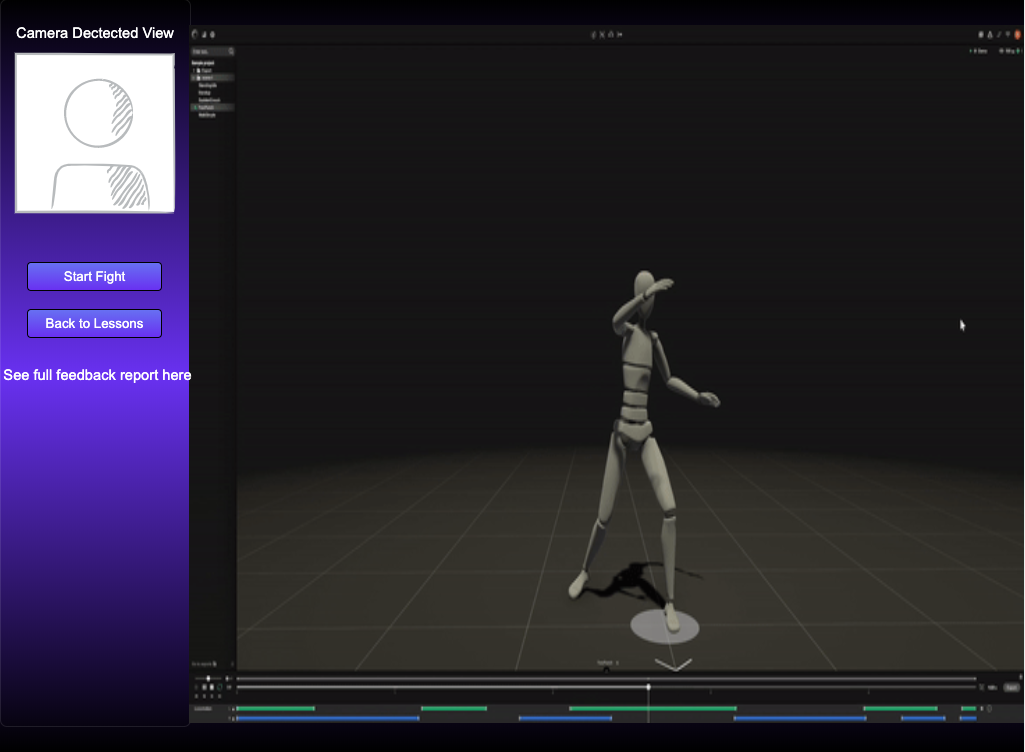
\includegraphics[scale=0.25]{images/Mockups/fight.png} \label{fig:fight} 
  }
  \caption{Practice and Fight Sessions} 
  \centering
  \label{fig:practiceFight}
\end{figure}


\subsection{Hardware/Communication Interfaces}
Since openpose will capture user's movements through a camera, a built-in camera or webcam is required. 
\\
All the hardware will require a connection with power source (9V battery) to power micro-controller, EMS (Electrical Muscle Stimulator) and tens machine.
\\
The Micro-controller will take decisions based on feature and pose vector to on and off some switches which control the tens machine and EMS.
\\
All the communication between hardware and software will be done serially, hence a serial communication cable will be required to transmit and receive data. 

\section{Use Cases}

Figure \ref{fig:usecase} shows the use case diagram of the project, which comprises of the functionalities of the system with respect to the user perspective. 


Following is a short description of the diagram: 


User can login/sign-up into the system and will be granted access after verification of credentials. After that they can either choose \textit{Train Mode} or \textit{Fight Mode}. The \textit{Train Mode} further includes tutorials and practice sessions. Both fight sessions and practice sessions provide user feedback indicating how well the user performed and how he can improve it. In addition to feedback, fight session also suggest tutorials based on areas the system thinks user has performed poorly. In case a user is fighting or practicing with haptics, they first need to calibrate the frequency and amplitude of the signal at which they are most comfortable.


\begin{figure}
    \centering
    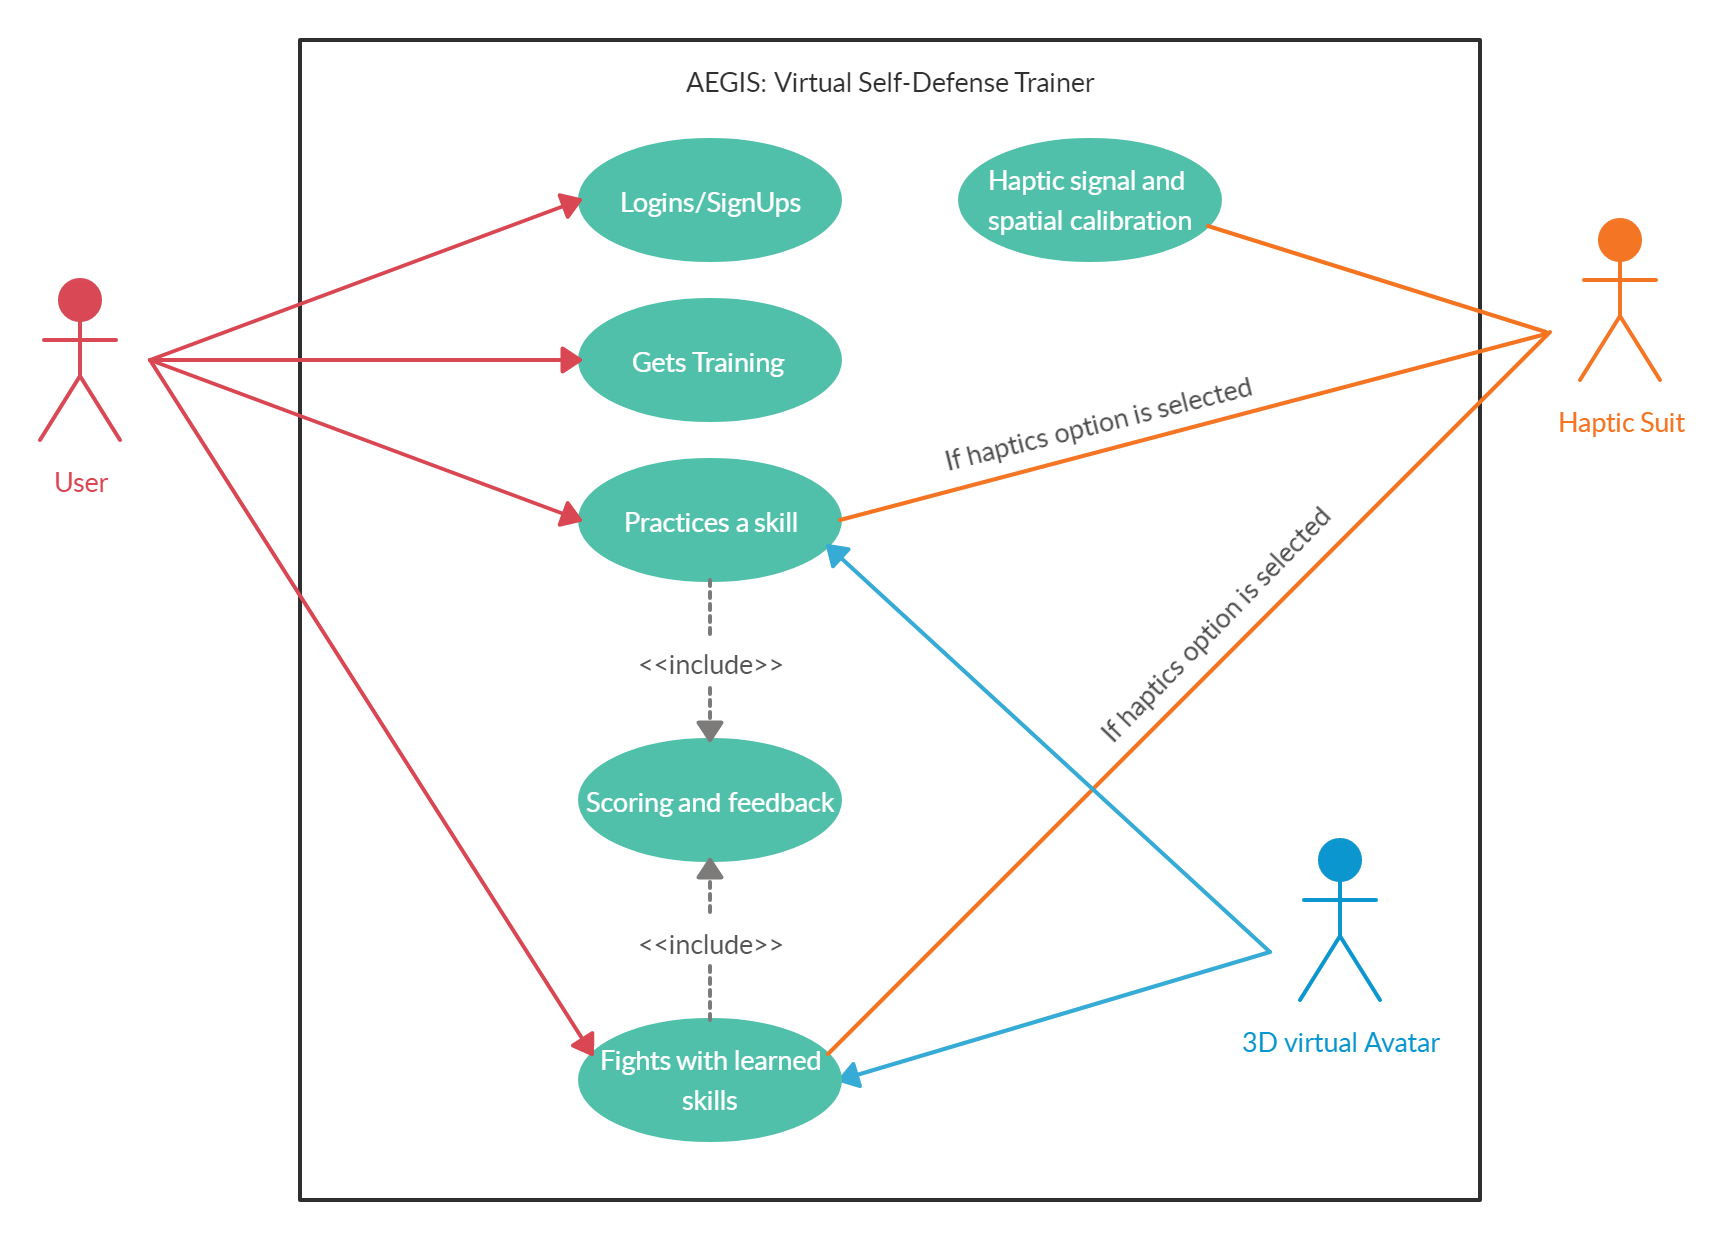
\includegraphics[scale=0.28]{images/UseCaseDiagram.png}
    \caption{Use Case Diagram}
    \label{fig:usecase}
\end{figure}


\section{Datasets}

There are no external datasets being used in this project. We have recorded our own videos for tutorials, and videos that serves as benchmark for pose evaluation and will be used in similarity comparison for pose classification. For validation of the system, we have created three classes of videos, having good, satisfactory and poor performance of the punch-block sequence.

\section{System Diagram}

\begin{figure}
    \centering
    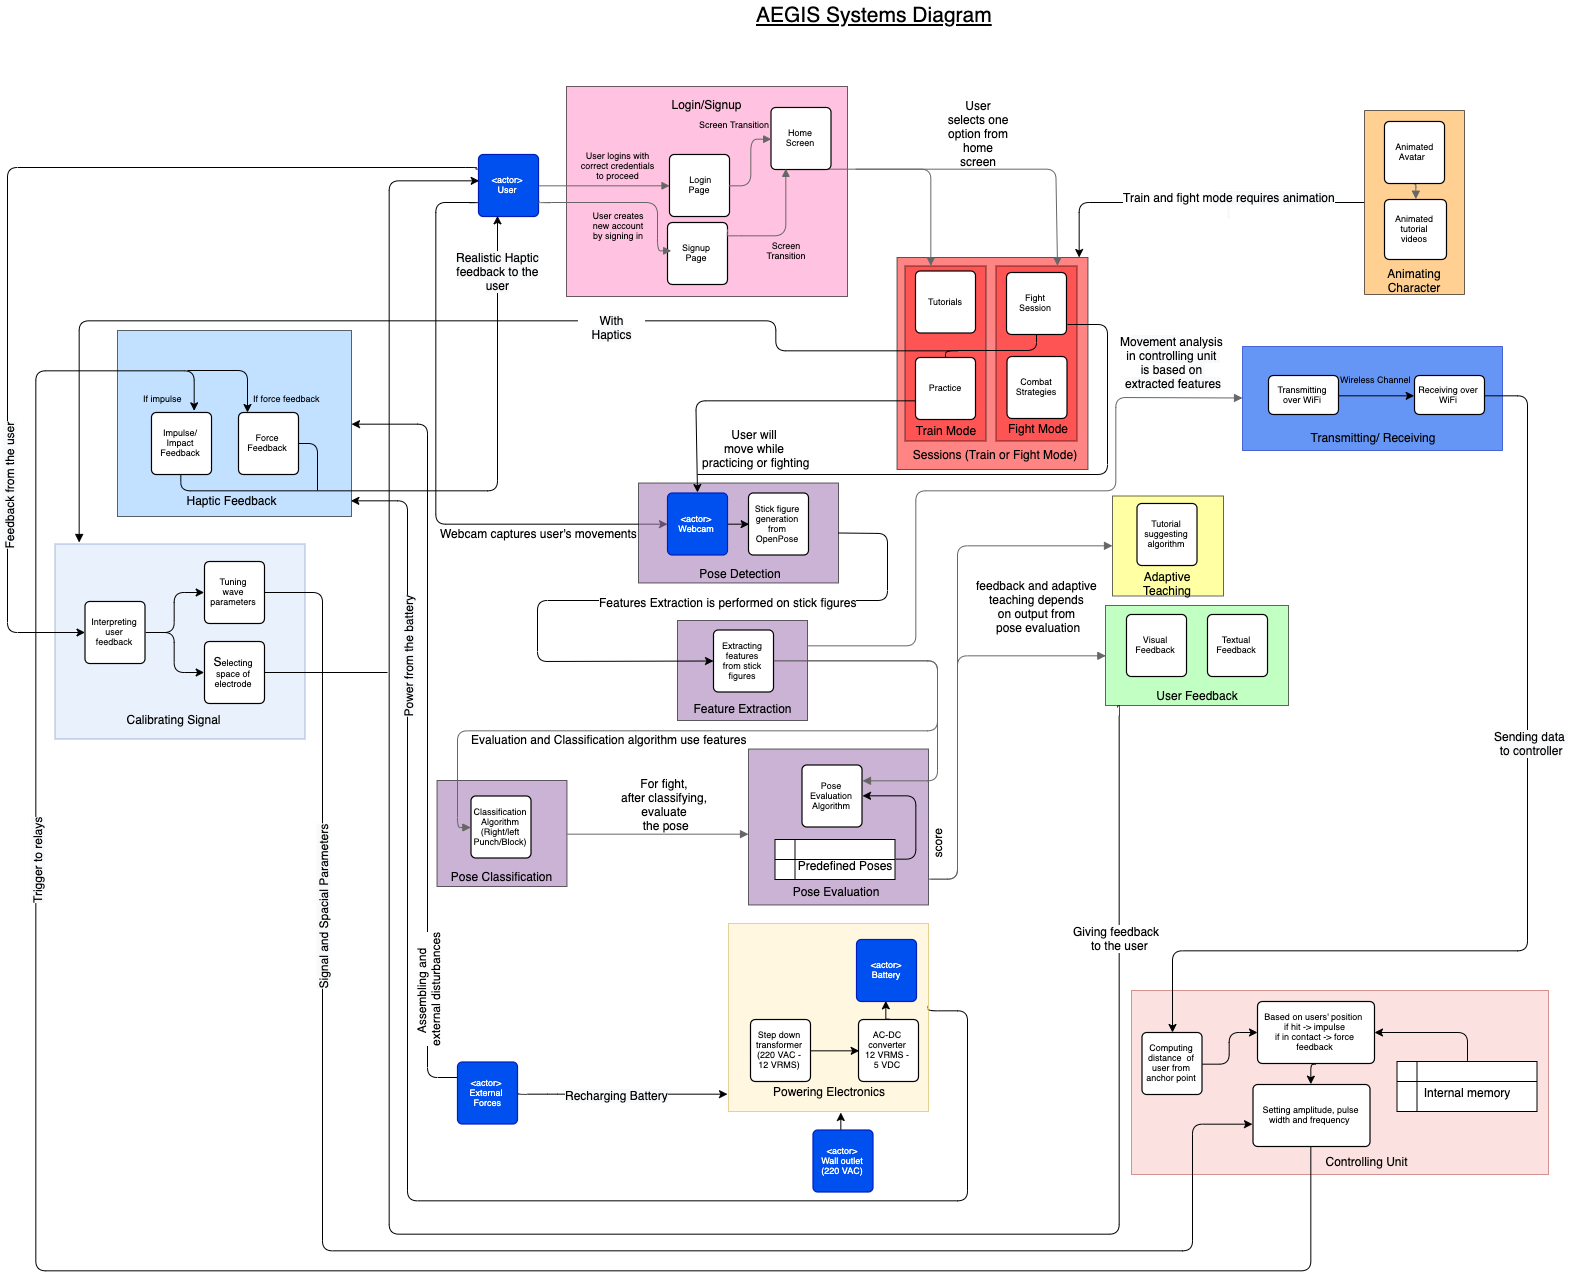
\includegraphics[scale=0.4]{images/SystemDiagram.png}
    \caption{System Diagram}
    \label{fig:systemDiagram}
\end{figure}

\clearpage

Figure \ref{fig:systemDiagram} shows the system diagram of our system which gives a high-level view of the different components of our system and the interactions between them. Each actor, component and the particular tools/technologies/libraries used to build it are described below.

\subsection{User}
User interacts with a few sub-systems in the main system. First of all, the user completes the sign-up or log-in step. This information is stored in the system's database and the process continues to either a \textit{Train Mode} or \textit{Fight Mode}. Hence, user outputs a selected mode, and in addition to that the user also outputs feedback to the calibration protocol if they choose to interact with haptics. The inputs to the user will be the haptic feedback, user feedback and visual display based on which it will interact with the system.

\subsection{Login/SignUp Module}
The input to this module are the user credentials (ID and password), and upon successful login/signup, the user can output a selection between train or fight mode.

\subsection{Animating Character Module}
This block is required to animate the avatar for the practice and fight session. This block will also animate user's body parts which will be in the view of the camera (like hands). 

\subsection{Sessions Module}
There are two modes that the user will select, either fight or train mode. Train mode is further divided into tutorials and practice sessions, while fight mode contains fight sessions along with avatar's combat strategies. Both the modes require animations from the animation module. 

\subsection{Calibrating Signal Module}
Before these sessions, if the user selects \textit{with haptics} then the haptics component needs to be calibrated. The calibration scheme consists of an automatic protocol that takes in user’s feedback as input to calibrate the parameters of wave (pulse width, frequency and amplitude of the EMS waves). These will be sent to the controlling unit and the controlling unit will tune in the parameters accordingly. Based on this, the output of the haptics will be modified, and the user will rate these modified sensations. This loop will continue until the sensation lies perfectly according to user's comfort. 

\subsection{Controlling Unit Module}
This block is comprised of primarily Arduino or any IoT platform. This will take in inputs over WiFi/cable from the Feature Extraction Module. Based on the feature vector, it will send in triggers and the parameters to the haptic block. This will make decisions as to which haptic signal to activate (impulse or force feedback). Based on distance of the user from the avatar it will activate the relays by comparing the distances with the pre-stored data and conditions in the memory. This also takes part in the calibration scheme where it gets information from the protocol and sets parameters accordingly.

\subsection{Haptic Feedback Module}
This block has two types of outputs, either a force feedback or an impulse feedback. The information about the wave parameters and when to activate comes directly from the Control Unit module. The output is directly exposed to the user. It makes the user feel the virtual environment.

\subsection{Transmission/Receiving Block}
This block gets the output from the feature extraction module and sends the feature vector to the control unit which makes decisions as described in Controlling Unit Module.

\subsection{Pose Detection Module}
This takes images from the webcam as inputs and outputs a series of time-dependent raw pose vectors in a csv file. This will be sent to the feature extraction module.

\subsection{Feature Extraction}
This module takes a series of time-dependent raw pose vectors in form of csv files as input and outputs features like velocity, acceleration, kinetic energy etc. This feature vector/tensor will be sent to the control unit and also to the pose classification block in the case of a fight session, before finally sending it to the pose evaluation module.

\subsection{Pose Evaluation Module}
This block gets input from the feature extraction block. This input feature vector is compared with the benchmark feature vector of predefined pose. Based on this comparison the score is given. The score is then sent to adaptive teaching block and the user feedback block.

\subsection{User Feedback Module}
This block gives feedback in natural language on based on the numerical score. The feedback will be sent to the display.

\subsection{Adaptive Teaching}
This component suggests the next tutorial based on the current performance score. The input is the score from pose evaluation and the outputs are the suggested tutorials that the user should practice more. 

\subsection{Powering Electronics}
This block recharges the battery and powers the entire circuitry including the haptic suit, the controlling unit, and the desktop (PC). 

\subsection{External Forces}
These are forces used for assembling in order to put the suit together. These external forces are at play when the user interacts with it whilst wearing the suit and recharging its battery (plug forces).




